\chapter{Problem Analysis}
%
The goal of this project is to develop a control strategy that can make an autonomous surface vessel suitable for survey tasks in water. More specifically, it should be able to perform bathymetric measurements.

In order to set up the requirements for the control system it is helpful to study a more concrete case in which bathymetric measurements are already in use and where improvements in measurement techniques are decried.

The Port of Aalborg provides such a case along with previously used bathymetric measurements, see \autoref{fig:bathymetricMapPortOfAalborg}. These measurements are used by the Port of Aalborg to guide ships safely through the port without hitting the bottom.

\begin{figure}[H]
  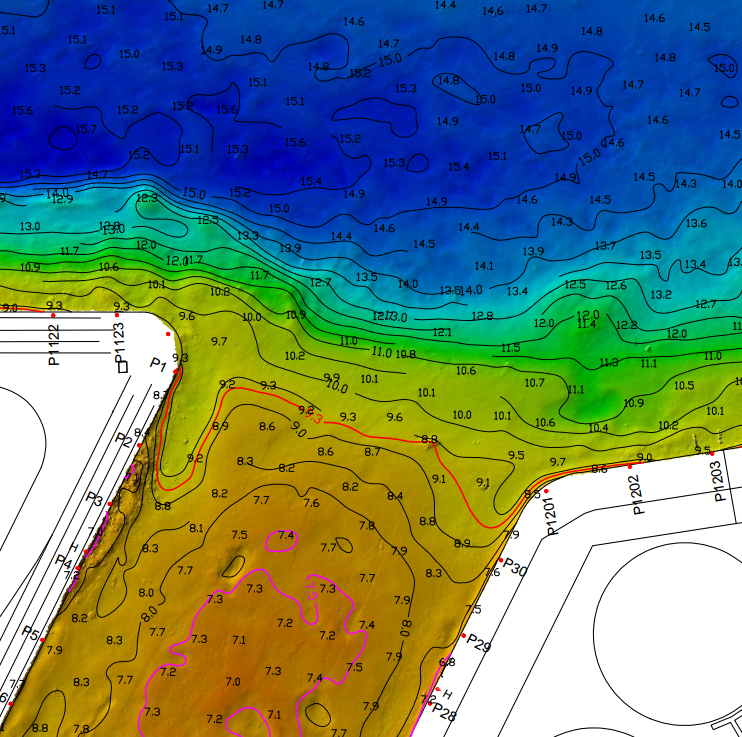
\includegraphics[width=0.5\textwidth]{figures/smallDebthMapAalborg}
  \caption{A cut from the full bathymetric map found in \autoref{app:bathymetricMapPortOfAalborg} provided by the Port of Aalborg \fxnote{cite port of aalborg}.}
  \label{fig:bathymetricMapPortOfAalborg}
\end{figure}

The depths of the port are in constant change due to shifting sands on the bottom. So while the bathymetric measurements helps in guiding the ships by the safest route they are not currently provided frequently enough that this can be done in the most optimal manner. If two ships are headed towards each other, one of them will be forced to wait in places where there is sure to be enough space for both in order to allow them to pass each other. This however is sometimes an unnecessary precaution, had there been more recent knowledge of the depths in the port.\fxnote{who do we source for this?}

The measurements are currently performed from a manned vessel on which a multi beam echo sounder is installed. Contrary to single beam echo sounders, the multi beam can sweep a wider area. It is still however a time consuming task.\fxnote{more specifically how often, one or more boats, what exact kind of multi beam echo sounder is used?}

It is therefore desired to automate the process, preferably with a smaller unmanned vessel. This will allow for more frequent bathymetric measurements and the efficiency of guiding ships through the Port of Aalborg can be improved.

The controller design must be able to track references provided by a path planer as well as rejecting disturbances such as possible wind or the effect of the waves. This requires a model of the disturbances to be included in the controller design along with a robust controller capable of handling model uncertainties.

The path planer must be able to design a route, in the form of waypoints\fxnote{not necessarily, is it not too early to decide?}, to reach all the positions needed to perform the different measurements required for the survey.

The accuracy and precision with which the route can be tracked has a significant impact on the efficiency of the system. The less closely the path is tracked, the more overlap of the echo sounder beam is required from each sweep in order to cover the entirety of the bottom.

The quality of the bathymetric measurements will also play part in determining the required overlap. Additionally other applications for the ASV would have requirements for the precision and accuracy provided by the control design. For these reasons and in order not to constrain the design to only one potential use, it is decided to set up some rather tight requirements for the system.

\section{Design Considerations}
The system design assumes that the sensor used to measure the bottom of the fjord is based on the current multibeam echosounder used by the Port of Aalborg, the multibeam echosounder SeaBat 7125 \cite{echoSounder}, which has a swath angle of 140$^\mathrm{o}$.

Based on the bathymetric map found in \autoref{app:bathymetricMapPortOfAalborg}, a minimum depth can be considered to estimate the width of the beam when it reaches the bottom. This width is used to plan the trajectory that the boat needs to follow to be able to reach all the points in a given area, see \autoref{chap:outerController}. In \autoref{fig:echosounder} a diagram of the echosounder's beam can be seen.

\begin{figure}[H]
    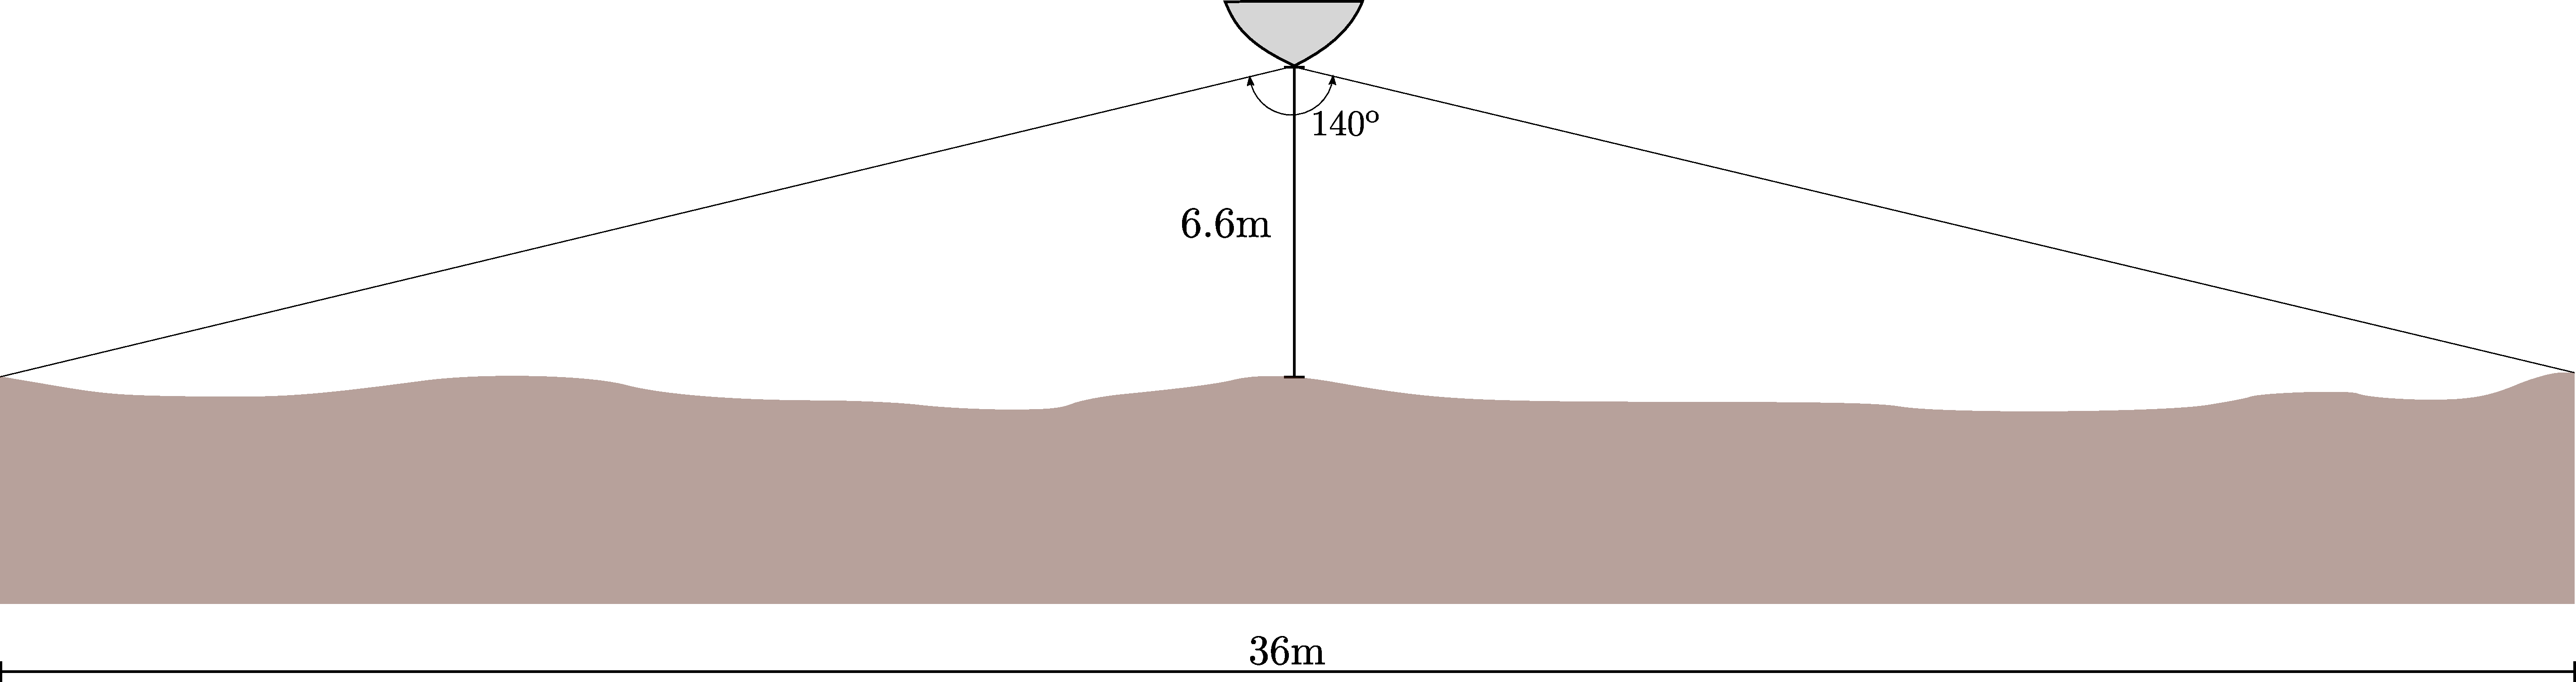
\includegraphics[width=0.9\textwidth]{figures/echosounder}
    \caption{Diagram of the echosounder's beam.}
    \label{fig:echosounder}
\end{figure}

\section{Functional Requirements} \label{sec:requirements}
To be able to design a working prototype some functional requirements must be set and verified at the end of the project once all the design has been carried out.
%
\begin{enumerate}
  \item It should be possible to select the area in which the bathymetric measurements are to be performed.
  \item A path planning algorithm should be able to plan a path within the selected area such that the bathymetric measurements can be performed.
  \item It should be possible to track the path laid out by the path planning algorithm.
  \item It should be possible to store the recorded data locally for extraction at the end of the survey.
  \item It should be possible to give the ASV a command to stop or call it back to land.
\end{enumerate}
%
The remainder of the problem analysis will go into how the functional requirements can be achieved. This will result in a set of technical requirements, which sets the perimeters of the design.






%\section{Technical Requirements}
%\fxnote{this section should be placed after analysis of sensors}
%Track position reference:\\
%- Summary of results of sensor capabilities\\
%- precision requirements for the control design\\
%- The bathymetry measurements are reliant on how much the boat tips, as it is single beam and measures shortest distance in the beam, some analysis must be done in this regard. Maybe it is necessary to stabilize the boat with floats on its sides. It would still be sensitive to waves, maybe the problem can be solved by measuring the tilt of the boat and mapping the measurements to the correct point in the inertial system having used beam and tilt angle to calculate vertical distance. This approach will put the measurements in a band around the path of the boat rather than in a straight line, question is if this is a good or a bad thing?
%
%Is it necessary to consider the water level on the day/time of the measurement? This is information which could be pulled from the Internet I think, either manually or, if the vessel has a connection, automatically.
%
%Record and store data:\\
%- Summary of results of data recordings (how much space is needed)\\
%- Space requirement for storing data\\
%- If chosen to send data back: requirement for communication\\
%
%Simple stop and call back commands:\\
%- communication requirement



